\documentclass[12pt,a4paper]{article}
\usepackage[utf8]{inputenc}
\usepackage{amsmath,amsfonts,amssymb}
\usepackage{graphicx}
\usepackage{hyperref}
\usepackage{geometry}
\usepackage{tabularx}
\usepackage{booktabs}
\usepackage{tikz}
\usepackage{float}
\usepackage{fancyhdr}
\usepackage{xcolor}
\usepackage{listings}

\geometry{margin=1in}
\pagestyle{fancy}
\fancyhf{}
\rhead{Meowcessor - ALU Wrapper Documentation}
\lhead{\today}
\cfoot{\thepage}

\definecolor{codegreen}{rgb}{0,0.6,0}
\definecolor{codegray}{rgb}{0.5,0.5,0.5}
\definecolor{codepurple}{rgb}{0.58,0,0.82}
\definecolor{backcolour}{rgb}{0.95,0.95,0.92}

\lstdefinestyle{mystyle}{
    backgroundcolor=\color{backcolour},   
    commentstyle=\color{codegreen},
    keywordstyle=\color{magenta},
    numberstyle=\tiny\color{codegray},
    stringstyle=\color{codepurple},
    basicstyle=\ttfamily\footnotesize,
    breakatwhitespace=false,         
    breaklines=true,                 
    captionpos=b,                    
    keepspaces=true,                 
    numbers=left,                    
    numbersep=5pt,                  
    showspaces=false,                
    showstringspaces=false,
    showtabs=false,                  
    tabsize=2
}
\lstset{style=mystyle}

\begin{document}

\title{\textbf{Meowcessor CPU Project}\\ \Large ALU Wrapper \& Dispatch Design Document}
\author{Aadi}
\date{\today}
\maketitle

\tableofcontents
\newpage

\section{Introduction}
This document details the architecture and implementation of the Arithmetic Logic Unit (ALU) wrapper for the \textbf{Meowcessor} RISC-V 32-bit CPU. The ALU wrapper unifies the project's individual arithmetic units—specifically the Kogge-Stone parallel-prefix adder, the Booth radix-4 multiplier, and the SRT radix-4 divider—behind a single, cohesive interface. 

The wrapper handles internal opcode decoding, dispatches operations to the correct sub-unit, manages multi-cycle operation handshaking, and routes the final results back to the execution pipeline.

\section{Architecture and Topology}
The ALU acts as a central multiplexer and orchestrator over several distinct execution units. Upon receiving a \texttt{start} pulse alongside a 4-bit internal \texttt{alu\_op}, the dispatch unit categorizes the operation as either \textbf{single-cycle} or \textbf{multi-cycle}.

\subsection{Sub-units}
\begin{itemize}
    \item \textbf{Kogge-Stone Adder (\texttt{Add}):} Purely combinational. The ALU reuses this block for \texttt{ADD}, \texttt{SUB} (computed as $a + \sim b + 1$), and signed/unsigned comparisons (\texttt{SLT}, \texttt{SLTU}), where the subtraction result is inspected for sign bit and carry-out flags.
    \item \textbf{Bitwise Logic \& Shifts:} Purely combinational blocks implementing native Verilog bitwise logic (\texttt{AND}, \texttt{OR}, \texttt{XOR}) and shifts (\texttt{SLL}, \texttt{SRL}, \texttt{SRA}).
    \item \textbf{Booth Multiplier (\texttt{booth\_radix4\_multiplier}):} A sequential unit with a latency of 17 cycles, responsible for \texttt{MUL} and \texttt{MULH}.
    \item \textbf{SRT Divider (\texttt{radix4\_srt\_divider}):} A sequential unit with a latency of approximately 18 cycles, responsible for \texttt{DIV}, \texttt{DIVU}, \texttt{REM}, and \texttt{REMU}.
\end{itemize}

\subsection{Topology Diagram}
The following is an abstract representation of the ALU routing topology:

\begin{figure}[H]
    \centering
    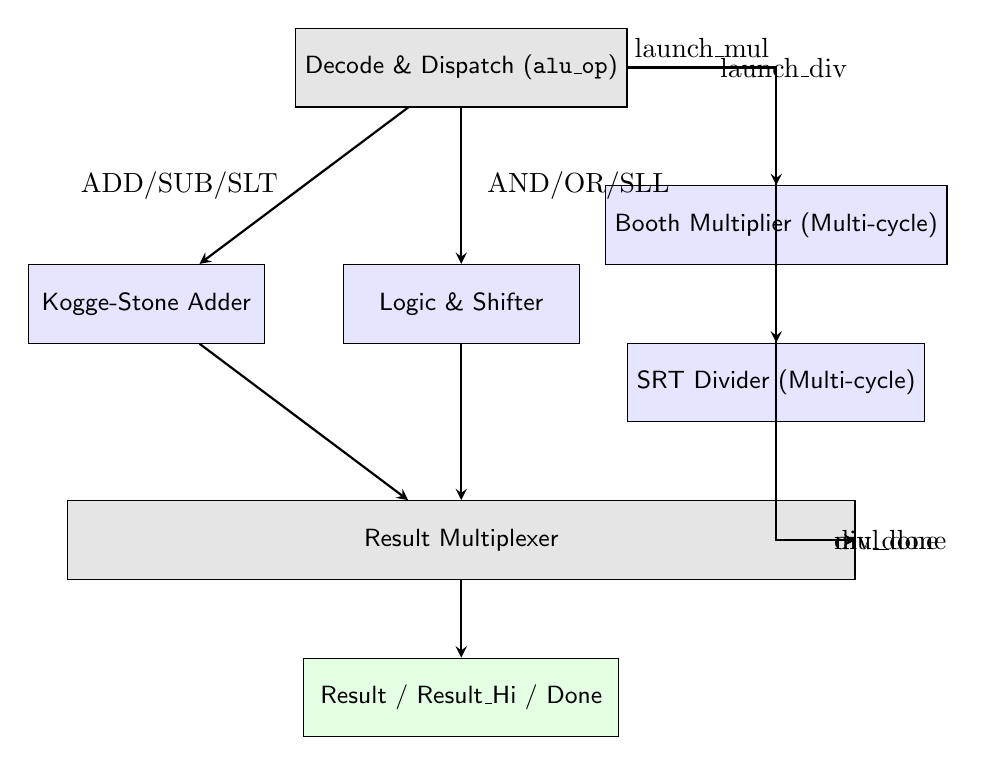
\begin{tikzpicture}[
        box/.style={draw, rectangle, minimum width=3cm, minimum height=1cm, text centered, font=\sffamily\small, fill=blue!10},
        arrow/.style={thick,->,>=stealth}
    ]
        % Nodes
        \node (op) [box, fill=gray!20] at (0, 6) {Decode \& Dispatch (\texttt{alu\_op})};
        
        \node (add) [box] at (-4, 3) {Kogge-Stone Adder};
        \node (log) [box] at (0, 3) {Logic \& Shifter};
        \node (mul) [box] at (4, 4) {Booth Multiplier (Multi-cycle)};
        \node (div) [box] at (4, 2) {SRT Divider (Multi-cycle)};
        
        \node (mux) [box, fill=gray!20, minimum width=10cm] at (0, 0) {Result Multiplexer};
        
        \node (out) [box, fill=green!10, minimum width=4cm] at (0, -2) {Result / Result\_Hi / Done};
        
        % Connections
        \draw [arrow] (op) -- (add) node[midway, left=2mm] {ADD/SUB/SLT};
        \draw [arrow] (op) -- (log) node[midway, right=2mm] {AND/OR/SLL};
        \draw [arrow] (op) -| (mul) node[near start, above] {launch\_mul};
        \draw [arrow] (op) -| (div) node[near start, right=1mm] {launch\_div};
        
        \draw [arrow] (add) -- (mux);
        \draw [arrow] (log) -- (mux);
        \draw [arrow] (mul) |- (mux) node[pos=0.75, right=1mm] {mul\_done};
        \draw [arrow] (div) |- (mux) node[pos=0.75, right=1mm] {div\_done};
        
        \draw [arrow] (mux) -- (out);
    \end{tikzpicture}
    \caption{ALU Internal Routing Topology}
\end{figure}

\section{Opcode Integration (\texttt{defines.v})}
To decouple the ALU from the complex RV32IM Instruction Decode stage, we map the standard RISC-V fields (\texttt{opcode}, \texttt{funct3}, \texttt{funct7}) into a compact 4-bit internal representation (\texttt{ALU\_OP\_*}). This acts as the exclusive command language for the ALU wrapper.

\begin{table}[H]
    \centering
    \begin{tabularx}{\textwidth}{@{} c c X l c @{}}
        \toprule
        \textbf{Internal Code} & \textbf{Decimal} & \textbf{Description} & \textbf{Execution Unit} & \textbf{Latency} \\
        \midrule
        \texttt{ALU\_OP\_ADD}  & 0  & Addition & Kogge-Stone Adder & 1 \\
        \texttt{ALU\_OP\_SUB}  & 1  & Subtraction & Kogge-Stone Adder & 1 \\
        \texttt{ALU\_OP\_AND}  & 2  & Bitwise AND & Logic Block & 1 \\
        \texttt{ALU\_OP\_OR}   & 3  & Bitwise OR & Logic Block & 1 \\
        \texttt{ALU\_OP\_XOR}  & 4  & Bitwise XOR & Logic Block & 1 \\
        \texttt{ALU\_OP\_SLL}  & 5  & Logical Left Shift & Shifter Block & 1 \\
        \texttt{ALU\_OP\_SRL}  & 6  & Logical Right Shift & Shifter Block & 1 \\
        \texttt{ALU\_OP\_SRA}  & 7  & Arithmetic Right Shift & Shifter Block & 1 \\
        \texttt{ALU\_OP\_SLT}  & 8  & Set Less Than (Signed) & Kogge-Stone Adder & 1 \\
        \texttt{ALU\_OP\_SLTU} & 9  & Set Less Than (Unsigned) & Kogge-Stone Adder & 1 \\
        \texttt{ALU\_OP\_MUL}  & 10 & Multiplication (Low) & Booth Multiplier & 17 \\
        \texttt{ALU\_OP\_MULH} & 11 & Multiplication (High) & Booth Multiplier & 17 \\
        \texttt{ALU\_OP\_DIV}  & 12 & Division (Signed) & SRT Divider & $\sim$18 \\
        \texttt{ALU\_OP\_DIVU} & 13 & Division (Unsigned) & SRT Divider & $\sim$18 \\
        \texttt{ALU\_OP\_REM}  & 14 & Remainder (Signed) & SRT Divider & $\sim$18 \\
        \texttt{ALU\_OP\_REMU} & 15 & Remainder (Unsigned) & SRT Divider & $\sim$18 \\
        \bottomrule
    \end{tabularx}
    \caption{Meowcessor ALU Internal Opcodes}
\end{table}

\section{Two-Phase Registered Dispatch (Timing Fix)}
A significant challenge encountered during integration was a delta-cycle race condition between the ALU wrapper's state machine and the internal state machines of the Multiplier/Divider.

\subsection{The Problem}
When the testbench (or ID stage) asserted \texttt{start = 1} for a single clock cycle, a naive combinational dispatch (\texttt{assign mul\_start = start \&\& is\_multicycle}) caused a race. On the rising clock edge, the ALU wrapper registered its \texttt{multicycle\_active} flag. Simultaneously, the sub-unit sampled \texttt{mul\_start}. The glitch on the combinational wire resolved before the sub-unit could reliably capture the start pulse, causing the multiplier to remain idle.

\subsection{The Solution}
The ALU utilizes a registered two-phase approach to guarantee a clean handshake.
\begin{enumerate}
    \item \textbf{Phase 1 (Cycle N):} The ALU detects \texttt{start == 1}. It asserts its internal \texttt{multicycle\_active} state and registers a launch request (e.g., \texttt{launch\_mul <= 1}).
    \item \textbf{Phase 2 (Cycle N+1):} The \texttt{launch\_mul} signal generates a clean, registered one-cycle pulse (\texttt{mul\_start <= 1}). The sub-unit safely samples this on Cycle N+2.
\end{enumerate}

This pattern adds exactly one cycle of latency to multi-cycle operations but guarantees robust synchronization across clock edges.

\section{Generated Gate-Level Hierarchy}
The ALU wrapper was synthesized using Yosys to verify elaboration and module connectivity. Below is the generated hierarchy schematic of the \texttt{alu} top module and its instantiations of the Kogge-Stone Adder, Booth Multiplier, and SRT Divider.

\begin{figure}[H]
    \centering
    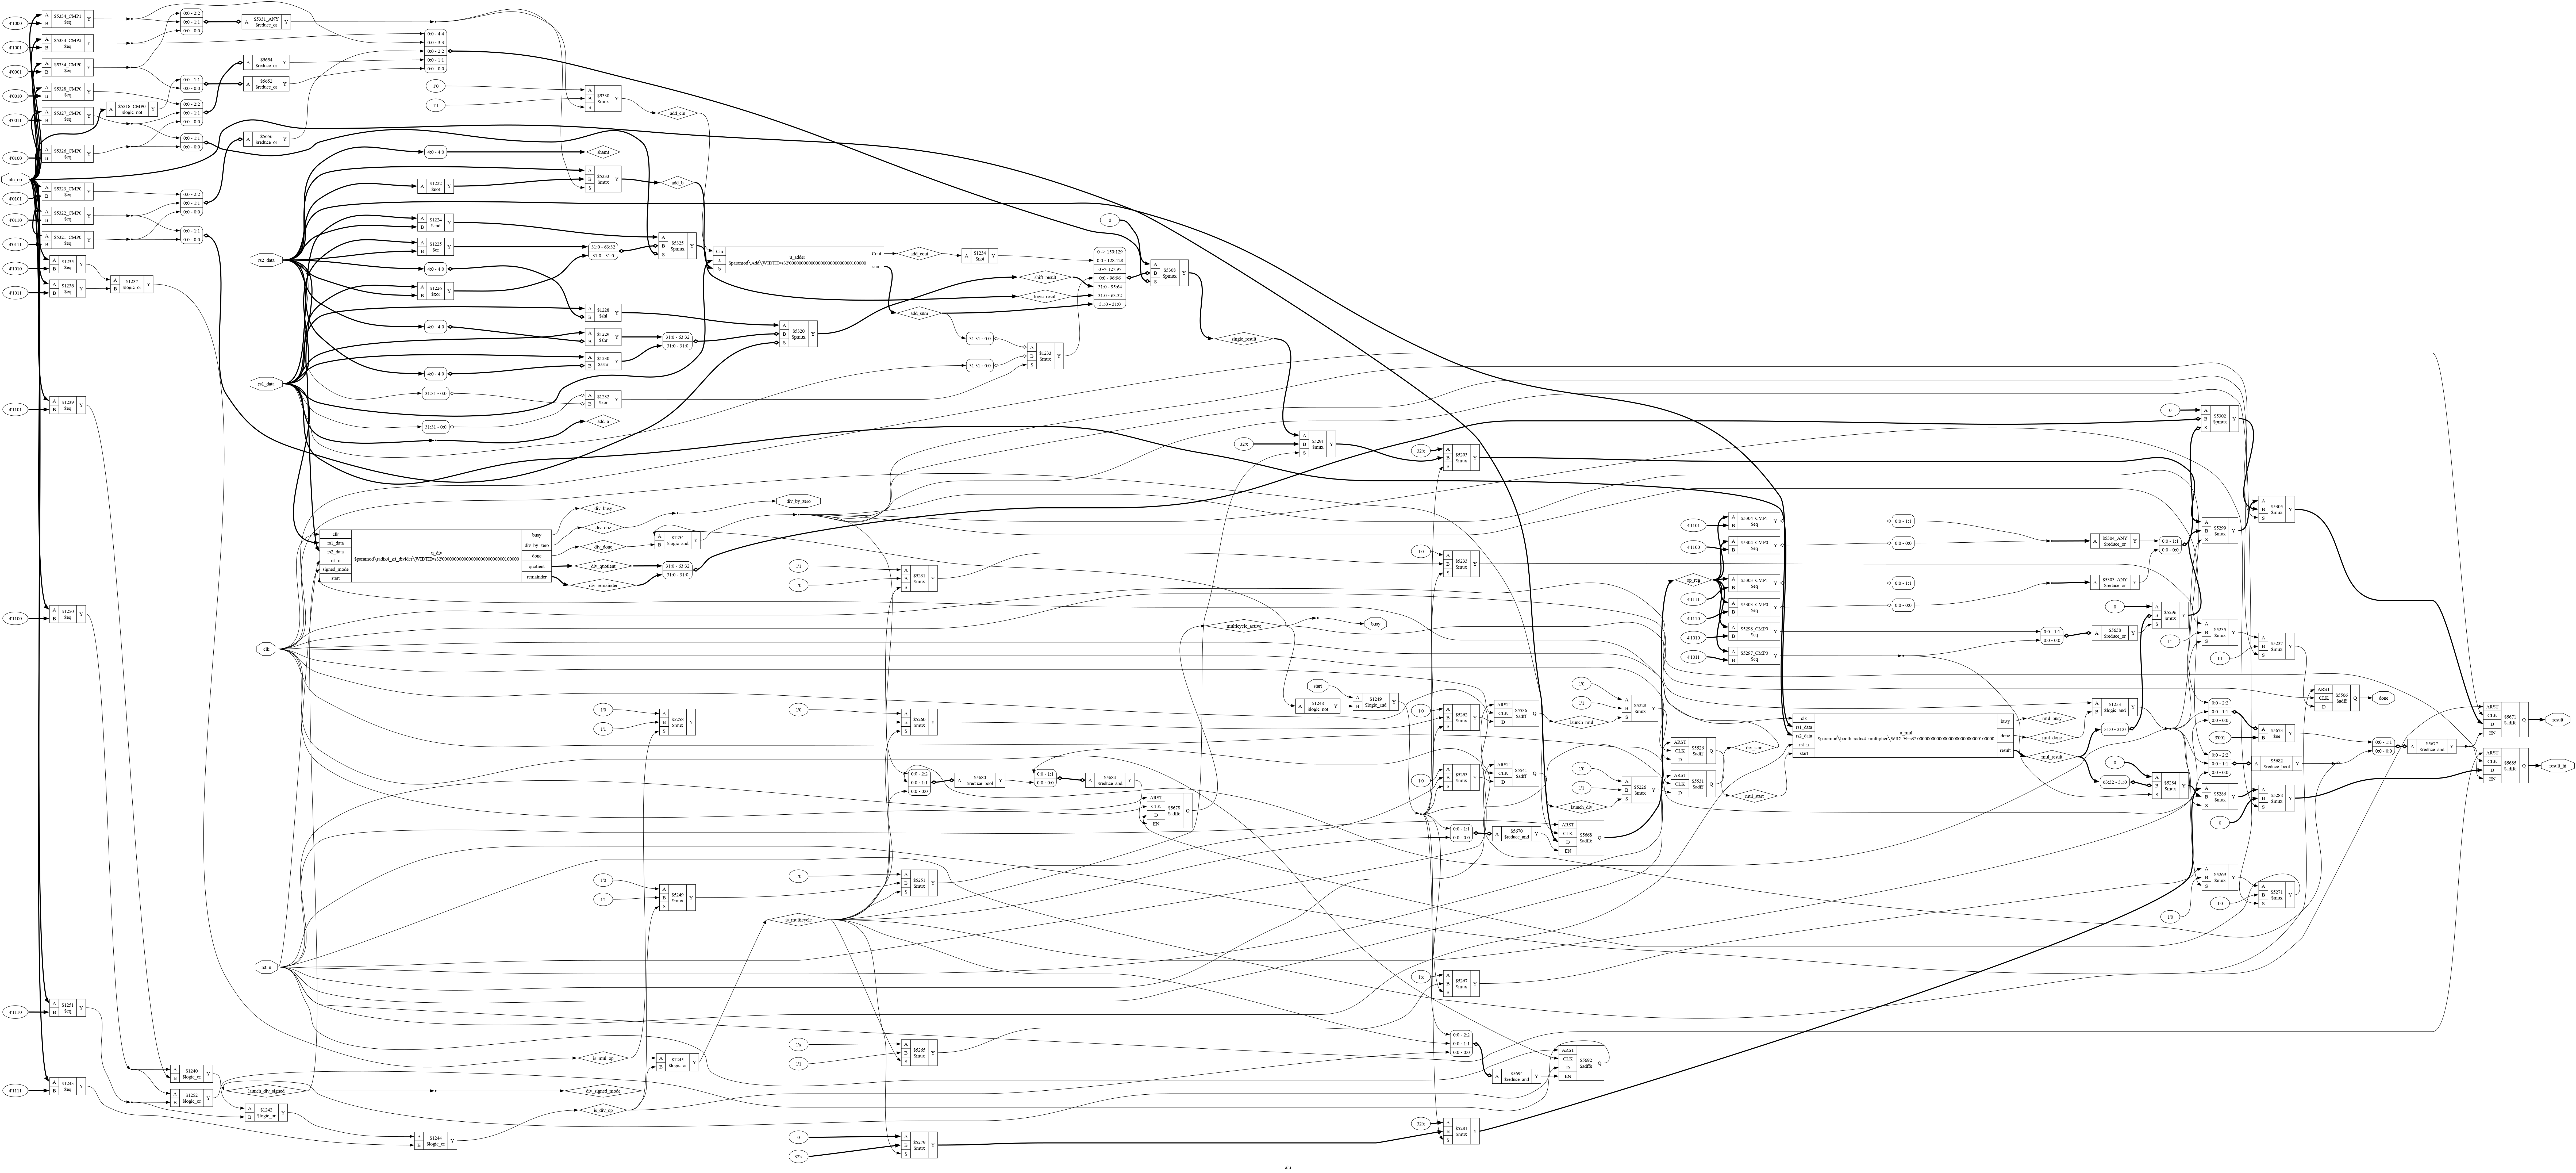
\includegraphics[width=\textwidth,height=0.45\textheight,keepaspectratio]{alu_hier.png}
    \caption{Yosys Generated Hierarchy Schematic}
\end{figure}

\section{Conclusion}
The completed ALU wrapper passes all 1,571 directed and randomized test vectors in the testbench (\texttt{alu\_tb.v}). The module is now ready to be integrated with the CPU's Register File and Instruction Decode (ID) pipeline stages.

\end{document}
